\documentclass{book}
\usepackage[default]{fontsetup}
\usepackage{graphicx,fullpage,supertabular}
\begin{document}


  \begin{center}
    {\LARGE The \texttt{fontsetup-nonfree} package}\\[1ex]
    \textit{by}\\[1ex]
    {\large Antonis Tsolomitis}\\
University of the Aegean\\ Department of Mathematics\\[1ex]
	  \textsc{3} May \textsc{2021}\\[1ex]
	  Version 1.02, \textsc{gpl3}
  \end{center}

  This package is part of the fontsetup package but for license issues it has been
  separated from the rest. For general information about the use of fontsetup check
  the file fontsetup-doc.pdf of the (free) fontsetup package. This package must
  be installed to access the commercial fonts that supports.

\bigskip

\textbf{Summary of installation steps to support all commercial fonts supported}

\medskip

\textit{Please note that Greek Small Caps for Linotype Palatino and MinionPro
  are supported only for} \verb|xelatex|.
 Users of \verb|lualatex| have to use custom commands as lua does not work with
  the \verb|ucharclasses| package.
\medskip

\begin{enumerate}
\item Install as system fonts the supplied \verb|fspmnscel.otf|
  and \verb|fsplpscel.otf| (in \verb|C:\Windows\Fonts\| on MS-Windows or in
  \verb|/home/user/.fonts/| in Linux or system-wide install as administrator)
\item Repeat the previous step for all MinionPro and MyriadPro fonts from the
  installation of the free Adobe Acrobat Reader.
\item Repeat the above for the MS-Garamond fonts (\verb|Gara.ttf|, \verb|Garabd.ttf|
  and \verb|Garait.ttf|) as well as for the Linotype Palatino fonts
  found in some versions of Microsoft Windows (\verb|palabi.ttf|, \verb|palab.ttf|,
  \verb|palai.ttf|, and \verb|pala.ttf|).
\item Repeat the above for the Cambria fonts (\verb|cambria.ttc|, \verb|cambriab.ttf|,
  \verb|cambriai.ttf|, \verb|cambriaz.ttf|).
\item Install the commercial Lucida fonts (if available) in your TeX tree.
%\item Install \verb|euler.otf| in your TeX tree from
%  here: \verb|https://github.com/khaledhosny/euler-otf|
\end{enumerate}

\bigskip




Samples of the supported commercial fonts follow.

\newpage

\begin{center}
{\Large Cambria and CambriaMath: option \verb|cambria|}\\
Cambria Fonts must be installed as system fonts\\[1cm] 
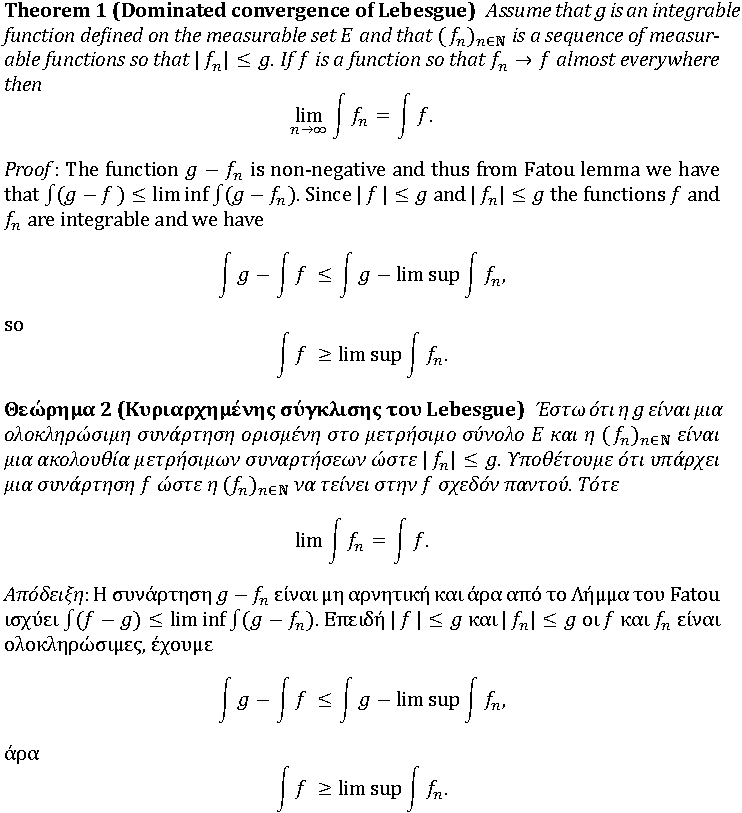
\includegraphics[scale=1.2]{fspsample-cambria.pdf}
\end{center}

\newpage

\begin{center}
{\Large Lucida and Lucida-Math (commercial): option \verb|lucida|}\\[1cm] 
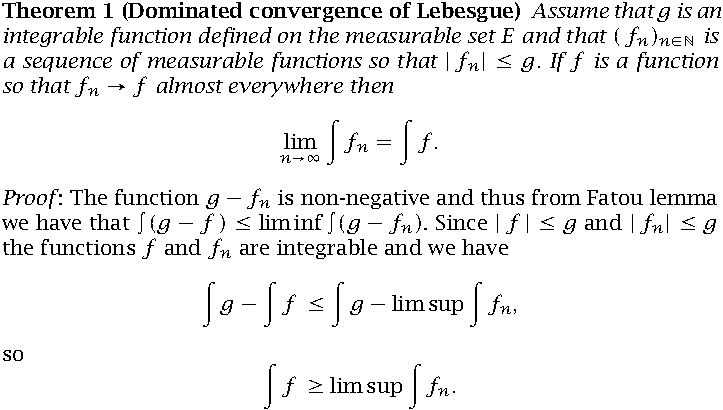
\includegraphics[scale=1.2]{fspsample-lucida.pdf}
\end{center}

\newpage

\begin{center}
{\Large MinionPro (commercial) and Stix2Math: option \verb|minion|}\\
MinionPro Fonts and the supplied fspmnscel.otf must
be installed as system fonts\\[1cm] 
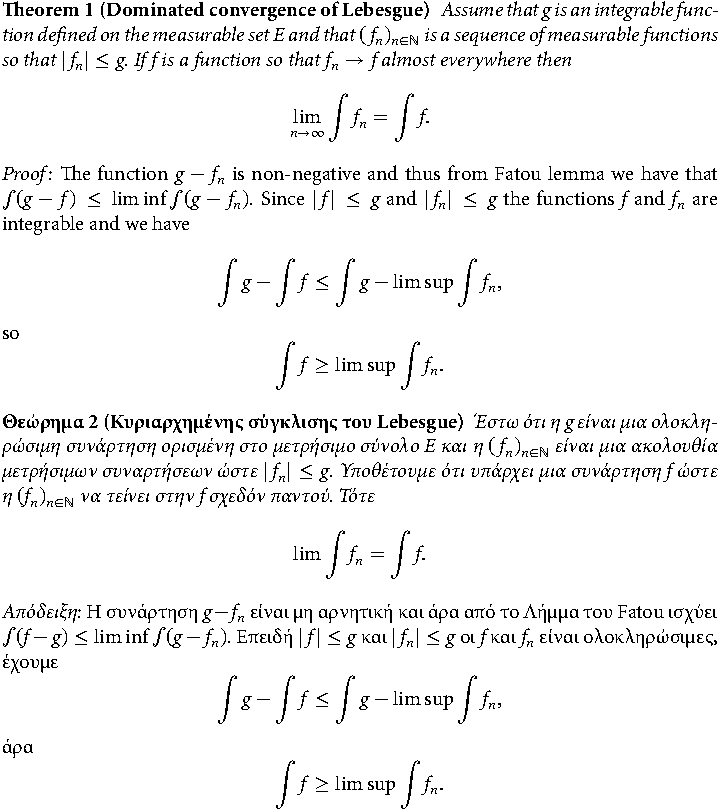
\includegraphics[scale=1.2]{fspsample-minion.pdf}
\end{center}

\newpage

\begin{center}
{\Large MS-Garamond (commercial) and Garamond-Math: option \verb|msgaramond|}\\
MS-Garamond Fonts must be installed as system fonts\\[1cm] 
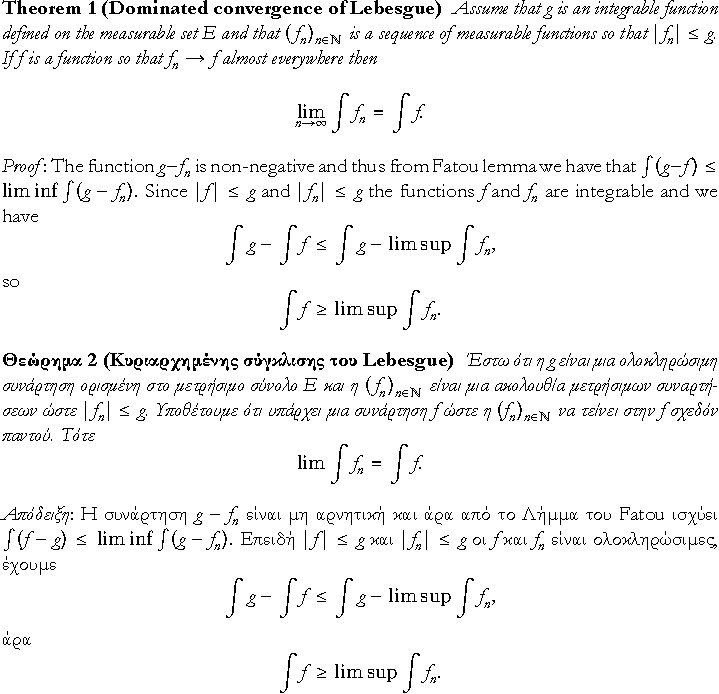
\includegraphics[scale=1.2]{fspsample-msgaramond.pdf}
\end{center}

\newpage

\begin{center}
{\Large Linotype Palatino (commercial) and texgyrepagella-math: option \verb|palatino|}\\
Linotype Palatino Fonts and the supplied fsplpscel.otf must be installed as system fonts\\[1cm] 
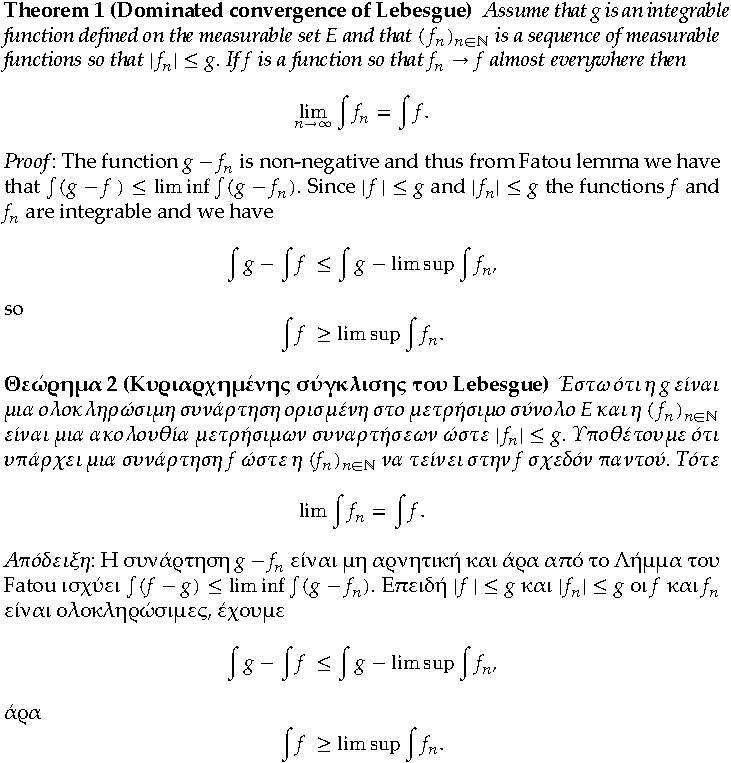
\includegraphics[scale=1.2]{fspsample-palatino.pdf}
\end{center}

\newpage


\end{document}
